\chapter{Auswertung}

\section{Benchmark Ergebnisse}

In der Abbildung \ref{fig:prototypeStreamingGraph} wird eine Übersicht über ein Standardtestdatensatz für das Zählen von Worten gezeigt.

\begin{figure}[htb!]
\centering
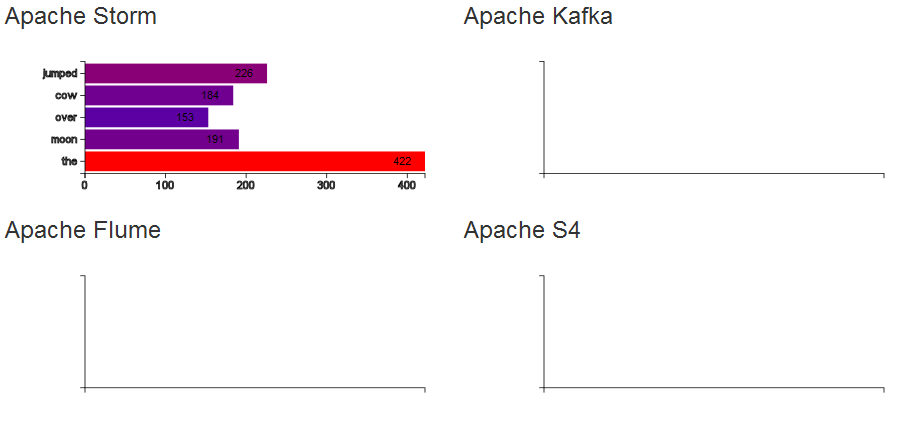
\includegraphics[width=1.0\textwidth]{bilder/PrototypeStreamingGraph.png}
\caption{Prototype Streaming Graph
\label{fig:prototypeStreamingGraph}}
\end{figure}


%STORM TRHOUGHPUT%
\begin{figure}
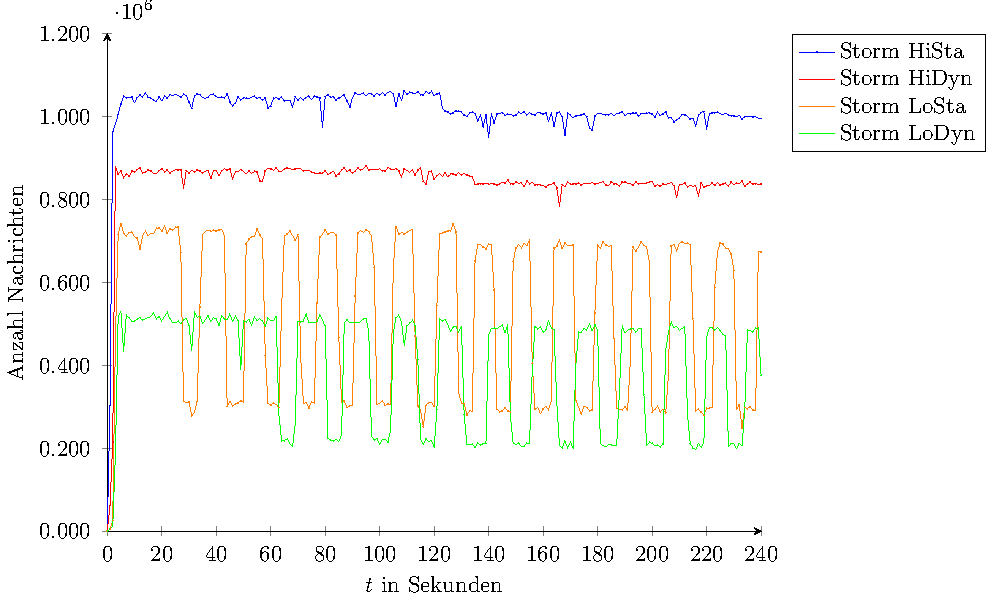
\includegraphics[width=0.97\textwidth]{plots/messungStormDurchsatz.pdf}
\caption{Messung Apache Storm Nachrichtendurchsatz
\label{fig:messungStormDurchsatz}}
\end{figure}
%STORM CPU%
\begin{figure}
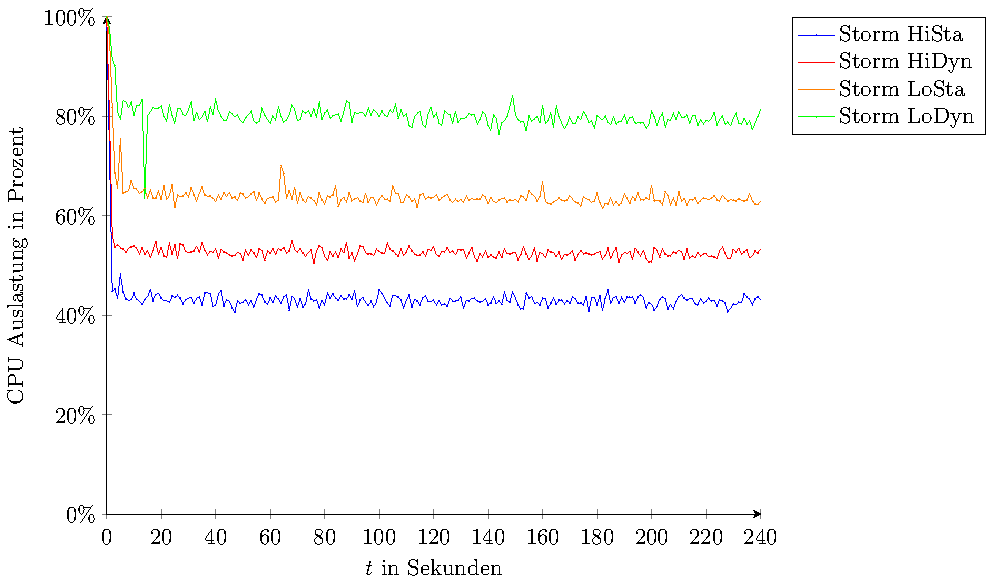
\includegraphics[width=0.97\textwidth]{plots/messungStormCpu.pdf}
\caption{Messung Apache Storm CPU Auslastung
\label{fig:messungStormCpu}}
\end{figure}


%KAFKA TRHOUGHPUT%
\begin{figure}
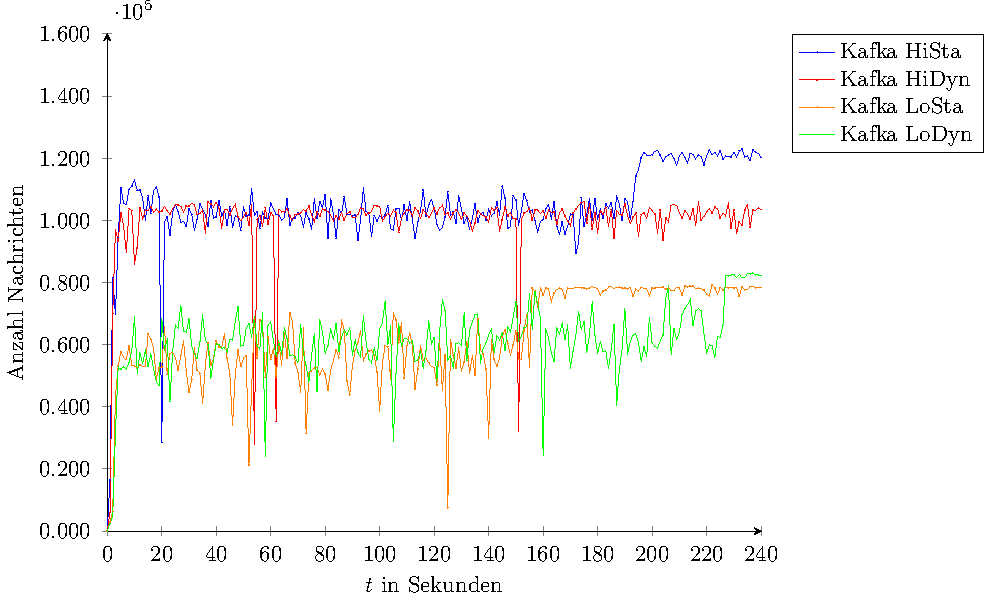
\includegraphics[width=0.97\textwidth]{plots/messungKafkaDurchsatz.pdf}
\caption{Messung Apache Kafka Nachrichtendurchsatz
\label{fig:messungKafkaNd}}
\end{figure}
%KAFKA CPU%
\begin{figure}
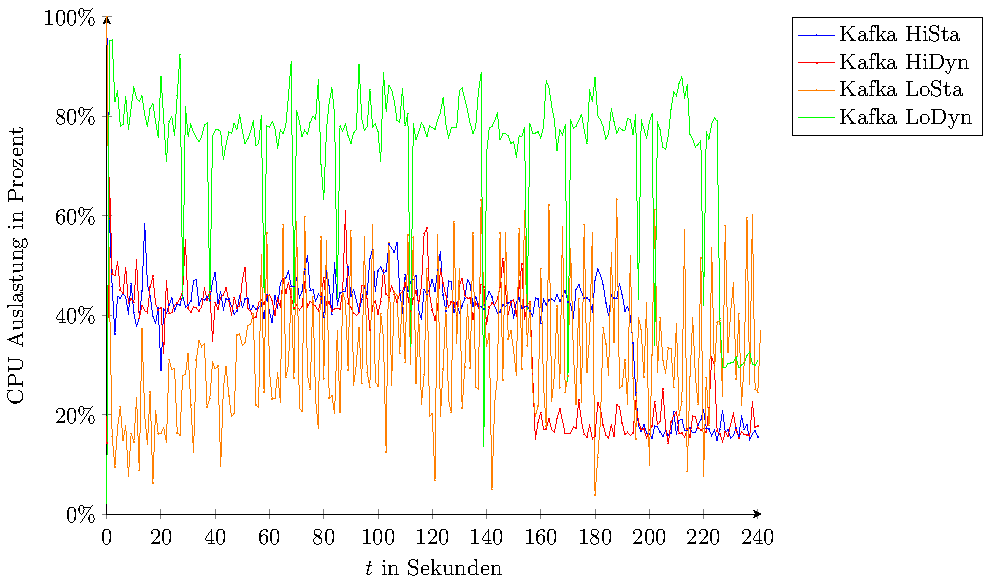
\includegraphics[width=0.97\textwidth]{plots/messungKafkaCpu.pdf}
\caption{Messung Apache Kafka CPU Auslastung
\label{fig:messungKafkaCpu}}
\end{figure}


%FLUME TRHOUGHPUT%
\begin{figure}
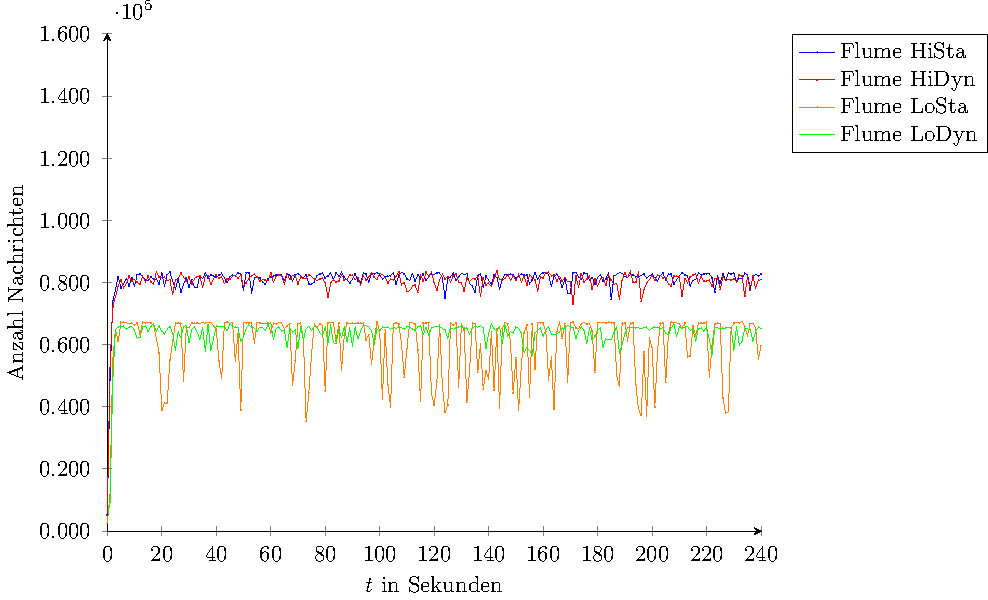
\includegraphics[width=0.97\textwidth]{plots/messungFlumeDurchsatz.pdf}
\caption{Messung Apache Flume Nachrichtendurchsatz
\label{fig:messungFlumeNd}}
\end{figure}
%FLUME CPU%
\begin{figure}
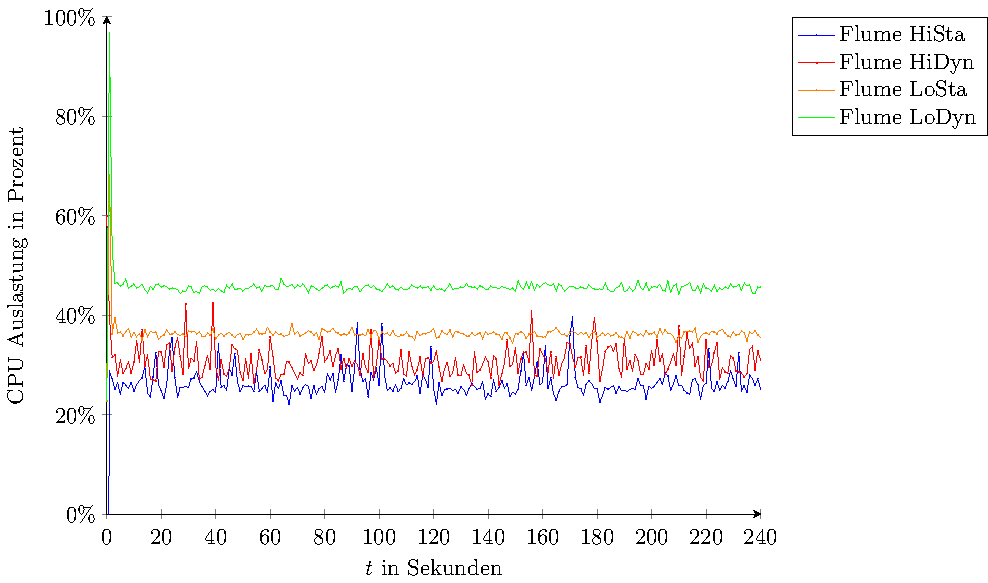
\includegraphics[width=0.97\textwidth]{plots/messungFlumeCpu.pdf}
\caption{Messung Apache Flume CPU Auslastung
\label{fig:messungFlumeCpu}}
\end{figure}


%S4 TRHOUGHPUT%
\begin{figure}
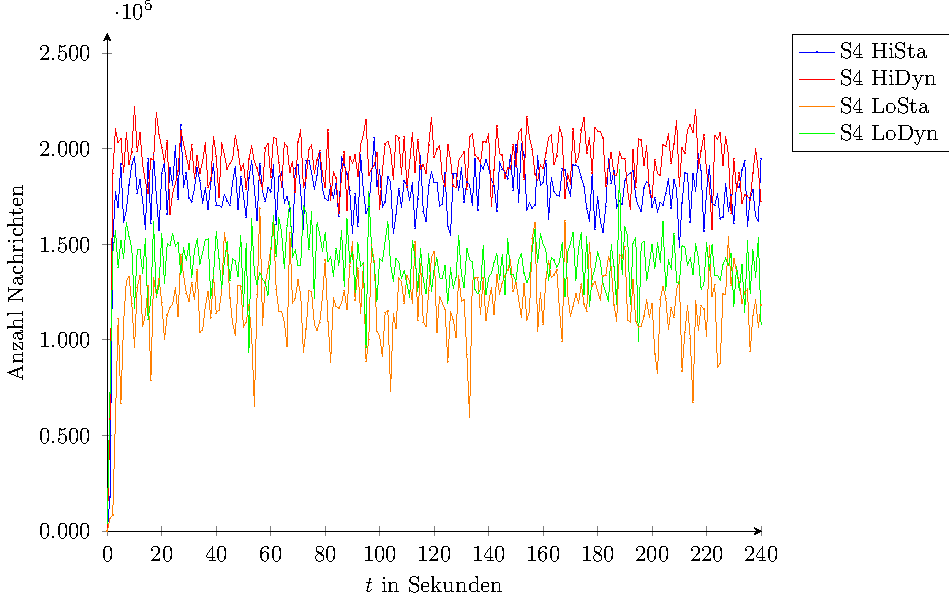
\includegraphics[width=0.97\textwidth]{plots/messungS4Durchsatz.pdf}
\caption{Messung Apache S4 Nachrichtendurchsatz
\label{fig:messungS4Nd}}
\end{figure}
%S4 CPU%
\begin{figure}
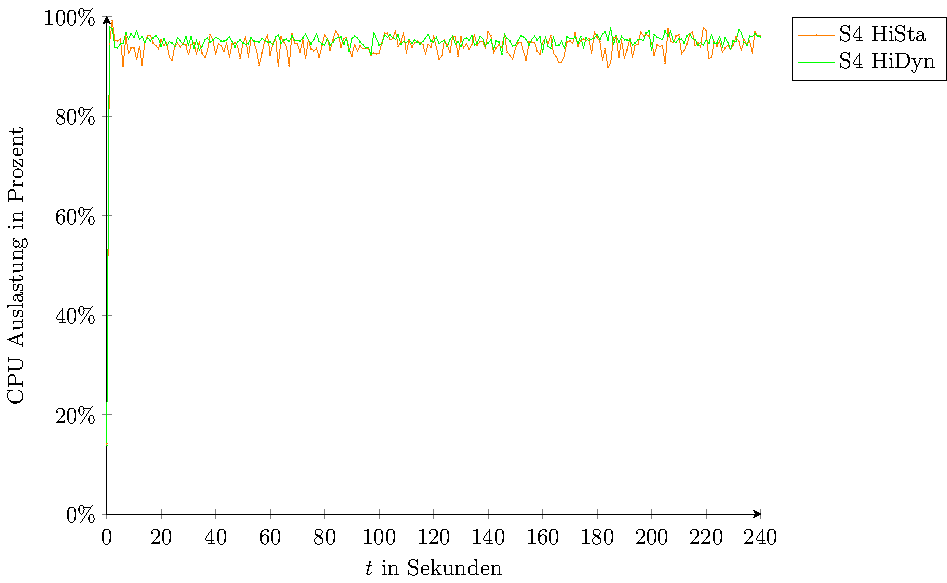
\includegraphics[width=0.97\textwidth]{plots/messungS4Cpu.pdf}
\caption{Messung Apache S4 CPU Auslastung
\label{fig:messungS4Cpu}}
\end{figure}



%Virtualbox RAW MEssung%
\begin{figure}
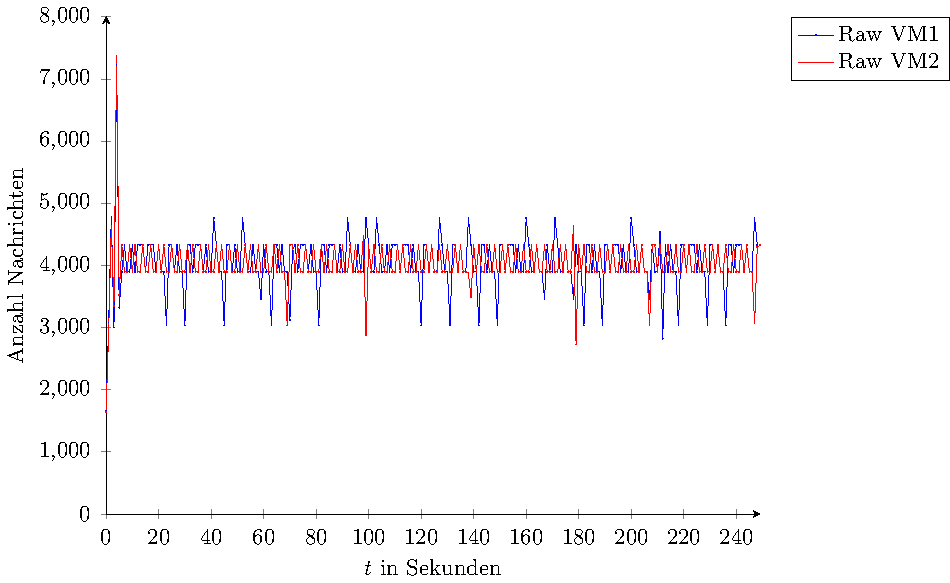
\includegraphics[width=1.0\textwidth]{plots/virtualBoxRaw.pdf}
\caption{Messung Nachrichtendurchsatz in Virtualbox
\label{fig:messungMaxNachrichten}}
\end{figure}






\section{Erkenntnis}


\begin{table}[tbp]
	\centering
		\begin{tabular}{@{}lll@{}} \toprule
			\textbf{Streaming Framework} & \textbf{Nachrichtendurchsatz pro S} & \textbf{CPU Auslastung in \%} \\ \midrule
			Apache Storm Hi & 732003 & 43 \\
			Apache Storm Lo & 546328 & 64 \\
			Apache Kafka Hi & 104571 & 39 \\
			Apache Kafka Lo & 62423 & 52 \\
			Apache Flume Hi & 80953 & 20 \\
			Apache Flume Lo & 60095 & 33 \\
			Apache S4 Hi & 177036 & 57 \\
			Apache S4 Lo & 118507 & 93 \\
			\bottomrule			
		\end{tabular}
	\caption{Übersicht Durchschnitte Streaming Frameworks CPU Auslastung und Nachrichtendurchsatz statisch}
	\label{tab:avgSta}
\end{table}

\begin{table}[tbp]
	\centering
		\begin{tabular}{@{}lll@{}} \toprule
			\textbf{Streaming Framework} & \textbf{Nachrichtendurchsatz pro S} & \textbf{CPU Auslastung in \%} \\ \midrule
			Apache Storm Hi & 810005 & 53 \\
			Apache Storm Lo & 506703 & 80 \\
			Apache Kafka Hi & 100009 & 41 \\
			Apache Kafka Lo & 61345 & 71 \\
			Apache Flume Hi & 80311 & 24 \\
			Apache Flume Lo & 63659 & 43 \\
			Apache S4 Hi & 192865 & 60 \\
			Apache S4 Lo & 139642 & 95 \\
			\bottomrule			
		\end{tabular}
	\caption{Übersicht Durchschnitte Streaming Frameworks CPU Auslastung und Nachrichtendurchsatz dynamisch}
	\label{tab:avgDyn}
\end{table}
